% Created 2021-10-06 mar 13:05
% Intended LaTeX compiler: pdflatex
%%% Local Variables:
%%% LaTeX-command: "pdflatex --shell-escape"
%%% End:
\documentclass[11pt]{article}
\usepackage[utf8]{inputenc}
\usepackage[T1]{fontenc}
\usepackage{graphicx}
\usepackage{grffile}
\usepackage{longtable}
\usepackage{wrapfig}
\usepackage{rotating}
\usepackage[normalem]{ulem}
\usepackage{amsmath}
\usepackage{textcomp}
\usepackage{amssymb}
\usepackage{listings}
\usepackage{capt-of}
\usepackage{hyperref}
\hypersetup{colorlinks=true, linkcolor=black}
\setlength{\parindent}{0in}
\usepackage[margin=1.1in]{geometry}
\usepackage[spanish]{babel}
\usepackage{mathtools}
\usepackage{palatino}
\usepackage{fancyhdr}
\usepackage{sectsty}
\usepackage{engord}
\usepackage{cite}
\usepackage{graphicx}
\usepackage{setspace}
\usepackage[compact]{titlesec}
\usepackage[center]{caption}
\usepackage{placeins}
\usepackage{tikz}
\usetikzlibrary{positioning}
\usetikzlibrary{bayesnet}
\usetikzlibrary{shapes.geometric}
\usetikzlibrary{decorations.text}
\usepackage{color}
\usepackage{amsmath}
\usepackage{minted}
\usepackage{pdfpages}

\def\inline{\lstinline[basicstyle=\ttfamily,keywordstyle={}]}

\titlespacing*{\subsection}{0pt}{5.5ex}{3.3ex}
\titlespacing*{\section}{0pt}{5.5ex}{1ex}
\author{José Antonio Álvarez Ocete\\ Francisco Javier Sáez Maldonado}
\date{\today}
\title{Introducción a Hadoop y Spark\\\medskip
\rarge Procesamiento de Datos a Gran Escala}

\newcommand{\I}{\mathbb{I}}
\newcommand{\ra}{\rangle}
\newcommand{\ra}{\rangle}

\begin{document}

\maketitle

\tableofcontents

Dividiremos esta práctica en 2 partes fundamentales. 

\begin{enumerate}
	
	\item En la primera, se concentrará en realizar diversas pruebas con los elementos más básicos de la programación en CUDA.
	\item En la segunda, TODO!!!!!!!!!!!
\end{enumerate}

\section{Parte 1: Programación GPGPU}

\subsection{Recursos de la GPU}

Para programar en GPU, el primer paso que debemos dar es conocer las características (y por tanto, los recursos) que el dispositivo del que disponemos nos ofrece. En este caso práctico, vamos a realizar las pruebas utilizando \href{https://colab.research.google.com/}{Google Colaboratory}. Google pone a disposición del usuario tanto GPUs como TPUs que son más que suficientes para realizar algunas pruebas. 

Lo primero que haremos es estudiar qué recursos tiene la GPU que nos ofrecen
\subsection{Suma de 2 vectores}
\subsection{Suma de 2 matrices}
\subsection{Stencil1d: Estudiar el efecto de la memoria compartida}

\section{Parte 2: Programación con QisKit: (Computación cuántica)}

Para esta parte de la práctica utilizaremos el \href{https://quantum-computing.ibm.com/composer}{Quantum Composer de IBM}. Puesto que el tenemos un número limitado de procesos a ejecutar (únicamente 5) veremos los resultados en el simulador sin llegar a medirlo en muchos casos.

\subsection{Puertas Cuánticas}

TODO: Añadir enunciado


\paragraph*{Puerta CNOT}

La única operación no trivial aplicable sobre un único bit es la negación: la puerta NOT. De la misma forma, es natural preguntarse cuál es el equivalente a la puerta NOT en el mundo cuántico. Dado que un qubit está descrito por dos amplitudes $\alpha$ y $\beta$:

\[
	|\varphi\ra = \alpha |0\ra + \beta |1\ra,
\]

la puerta NOT será un intercambio entre las posiciones de estas amplitudes, obteniéndose así:

\[
	|\varphi\ra = \beta |0\ra + \alpha |1\ra.
\]

La matriz unitaria que describe esta transformación es sencilla:

\[
X = \frac{1}{\sqrt 2}
\begin{pmatrix}
	0 & 1 \\
	1 & 0 
\end{pmatrix}
\]

Vemos la implementación de esta puerta en el Quantum Composer de IBM:

\begin{figure}[H]
	\centering
	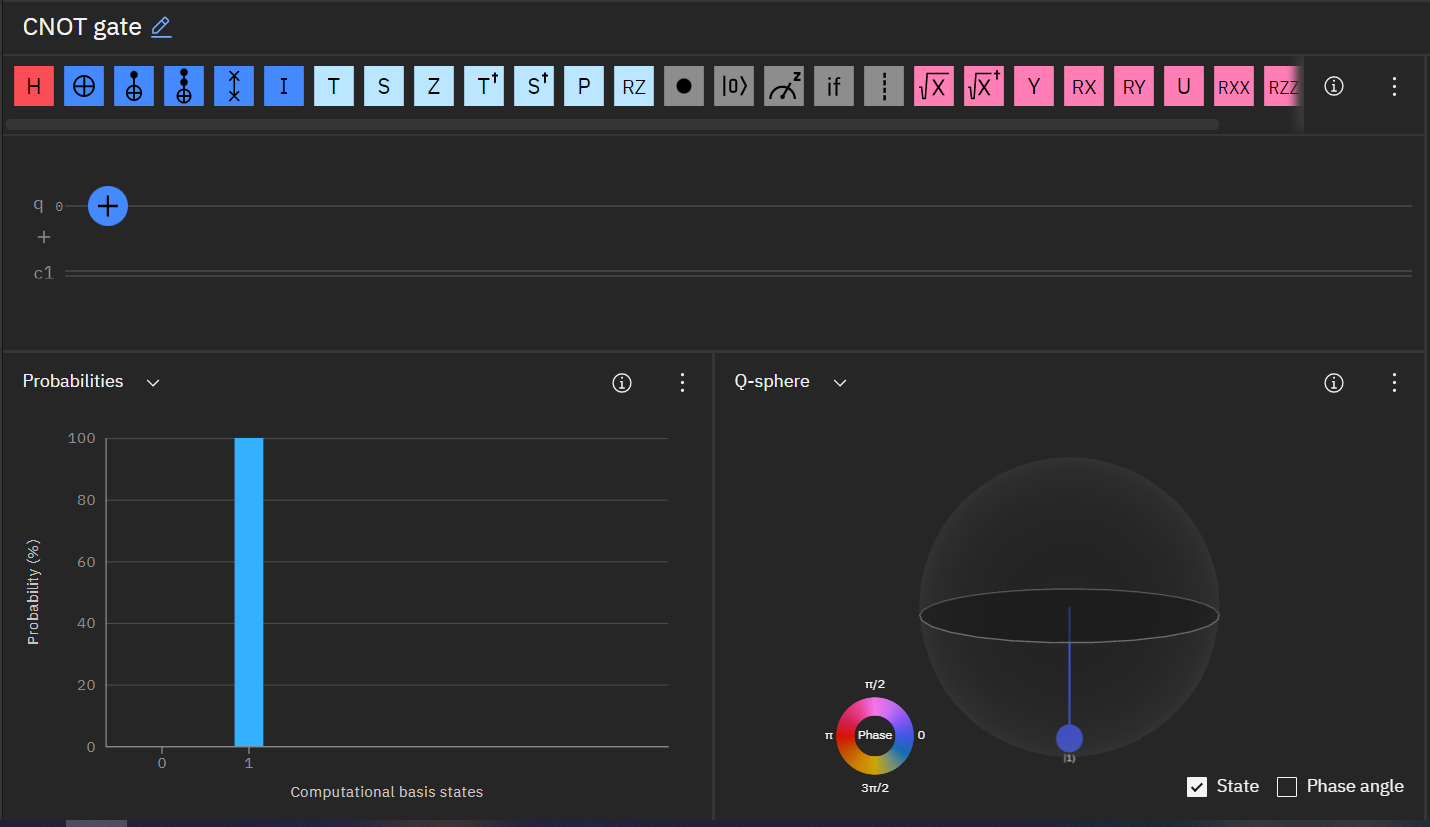
\includegraphics[scale=0.4]{figures/gate-x.png}
	\caption{Circuito con puerta de Hadamard}
\end{figure}

Recordemos que en el Quantum Composer de IBM todos los qubits empiezan siempre en el estado $|0\ra$. Tras aplicarlo a nuestro qubit una puerta $X$ obtendremos $|1\ra$.

\paragraph*{Puerta Hadamard}

Finalmente presentamos la puerta de Hadamard para un único bit. Está descrita por la siguiente matriz unitaria:

\[
	H_1 = \frac{1}{\sqrt 2}
	\begin{pmatrix}
		1 & 1 \\
		1 & -1 
	\end{pmatrix}
\]

Uno de sus usos más comunes es la superposición de qubits. Si aplicamos esta puerta al estado $|0\ra$ obtenemos el estado de Bell:

\[
	H|0\ra = \frac{1}{\sqrt 2} |0\ra + \frac{1}{\sqrt 2} |1\ra = |+\ra
\]

Mientras que si se la aplicamos al estado $|1\ra$ obtenemos:

\[
	H|1\ra = \frac{1}{\sqrt 2} |0\ra - \frac{1}{\sqrt 2} |1\ra = |-\ra
\]

Que también supone una superposición exacta de $|0\ra$ y $|1\ra$ puesto que $|1/\sqrt 2|^2 = |-1/\sqrt 2|^2 = 1/2$.

Podemos estudiar el comportamiento de esta puerta utilizando el Quantum Composer de IBM:

\begin{figure}[H]
	\centering
	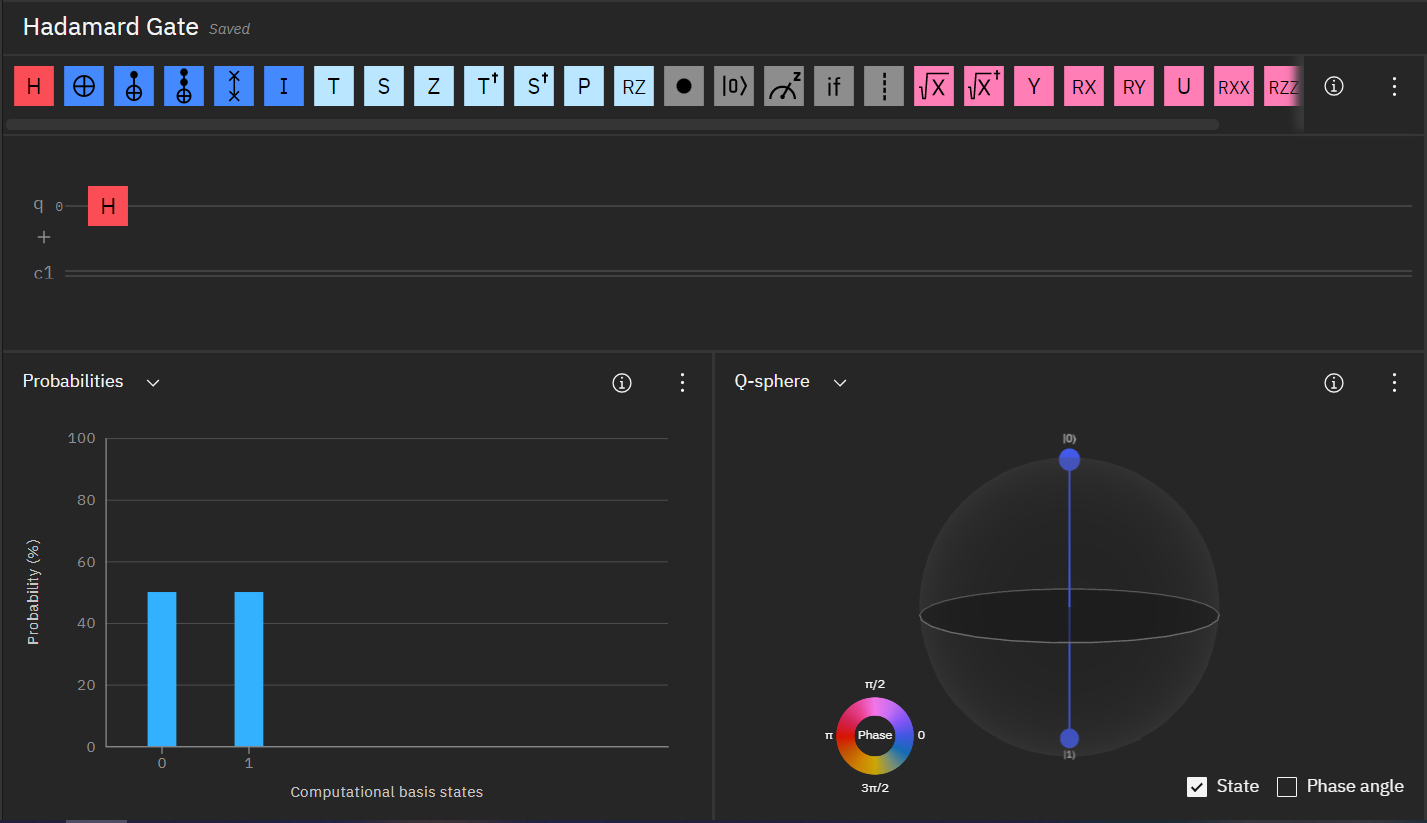
\includegraphics[scale=0.4]{figures/gate-hadamard.png}
	\caption{Circuito con puerta de Hadamard}
\end{figure}

Mirando tanto la \href{URL}{esfera de Bloch} como las probabilidades vemos que tenemos la misma probabilidad de medir $0$ y $1$.

\paragraph*{Puertas de Pauli}

Un conjunto particularmente relevante de puertas son las descritas por las \text{matrices de Pauli}:

\[
X =
	\begin{pmatrix}
		0 & 1 \\
		1 & 0 
	\end{pmatrix}; \quad
	Y =
	\begin{pmatrix}
		0 & -i \\
		i & 0 
	\end{pmatrix}; \quad
	Z =
	\begin{pmatrix}
		1 & 0 \\
		0 & -1 
	\end{pmatrix}
\]

Ya conocemos la matriz $X$, descrita también como la puerta NOT quántica.

\paragraph*{Puertas $T$}

La puerta $\pi/8$, normalmente descrita por la letra $T$, es una \emph{puerta de fase}. Las puertas de fase son un tipo especial de puertas cuánticas que llevan $|0\ra \mapsto |0\ra$ y $|1\ra \mapsto e^{i\phi}|1\ra$, donde $\phi$ es un ángulo de giro. El término $e^{i\phi}$ se denomina \emph{fase} y no afecta a los resultados de las mediciones $0$ y $1$. En particular, la puerta $T$ cumple $\phi = \pi/4$, y la puerta $Z$ de Pauli es una puerta fase con $\phi = \pi/2$:

\[
	T =
	\begin{pmatrix}
		1 & 0 \\
		0 & e^{i\frac{\pi}{4}}
	\end{pmatrix}; \quad
	Z =
	\begin{pmatrix}
		1 & 0 \\
		0 & e^{i\frac{\pi}{2}} = -1
	\end{pmatrix}
\]

En computación clásica, uno de los resultados básicos más relevante es que cualquier función booleana puede describirse utilizando únicamente las puertas clásicas AND, OR y NOT. De la misma forma, en computación cuántica se obtiene siguiente resultado

\begin{theorem}
	Toda matriz unitaria puede aproximarse con una combinación de puertas Hadamard, CNOT y $\pi/8$.
\end{theorem}

Esto es, todo circuito cuántico puede describirse utilizando únicamente dichas puertas.

\subsection{Generación de números aleatorios con un Computador Cuántico}

TODO: añadir enunciado

Sabemos que utilizando la puerta de Hadarmad $H$ explicada en el apartado anterior ponemos un qubit $|0\ra$ en superposición:

\[
	H|0\ra = \frac{1}{\sqrt 2} |0\ra + \frac{1}{\sqrt 2} |1\ra
\]

Si ahora medimos este qubit obtendremos $|0\ra$ con probabilidad $|1/\sqrt 2|^2 = 1/2$, y $|1\ra$ con probabilidad $1/2$. Esto es, hemos creado un generador de bits aleatorios utilizando un único qubit. Para crear un generador de 3 bits utilizaremos un sistema de 3 qubits. Inicialmente en el estado $|000\ra$, aplicaremos una puerta Hadamard a cada qubit de forma independiente, poniendo así cada qubit en superposición:

\[
	\hat H_3|000\ra = \frac{|000\ra + |001\ra + |010\ra + |011\ra + |100\ra + |101\ra + |110\ra + |111\ra}{\sqrt 8} |0\ra
\]

Donde la puerta $H_3$ tranformación de Hadamard para tres qubits. Se puede definir recursivamente de la siguiente forma:

\[
	H_m = H_1 \times H_{m-1}, H_1 = \frac{1}{\sqrt 2}
	\begin{pmatrix}
		1 & 1 \\
		1 & -1 
	\end{pmatrix}
\]

Así obtenemos la puerta Hadamard para tres qubits:

\[
	H_3 = \frac{1}{2^{3/2}}
	\begin{pmatrix}
		1 & 1 & 1 & 1 & 1 & 1 & 1 & 1 \\
		1 & -1 & 1 & -1 & 1 & -1 & 1 & -1 \\
		1 & 1 & -1 & -1 & 1 & 1 & -1 & -1 \\
		1 & -1 & -1 & 1 & 1 & -1 & -1 & 1 \\
		1 & 1 & 1 & 1 & -1 & -1 & -1 & -1 \\
		1 & -1 & 1 & -1 & -1 & 1 & -1 & 1 \\
		1 & 1 & -1 & -1 & -1 & -1 & 1 & 1 \\
		1 & -1 & -1 & 1 & -1 & 1 & 1 & -1
	\end{pmatrix}
\]

Pasamos a realizar un estudio empírico del circuito diseñado. Lo implementamos utilizando el Quantum Composer de IBM:

\begin{figure}[H]
	\centering
	\includegraphics[scale=0.8]{figures/3bit_rand.png}
	\caption{Circuito de generación de números aleatorios con 3 bits}
\end{figure}

Este simple circuito cuántico pone todos los qubits en superposición y después mide el resultado. En la parte inferior de la imagen vemos como tenemos la misma probabilidad de obtener cualquiera de los posibles resultados. Esto es, cualquiera de los números del $0$ al $7$, tomando así un número aleatorio de 3 bits. Añadimos tres medidas, una para cada qubit, y ejecutamos el circuito resultante utilizando un simulador de 

\begin{figure}[H]
	\centering
	\includegraphics[scale=0.8]{figures/3bit_rand_result.png}
	\caption{Resultados de la simulación con 1024 ejecuciones}
\end{figure}

Como podemos ver en la gráfica, obtenemos una probabilidad similar de medir cada uno de los posibles resultados.

\subsection{Entrelazamiento}

En este apartado explicaremos en detalle el siguiente circuito cuántico:

\begin{figure}[H]
	\centering
	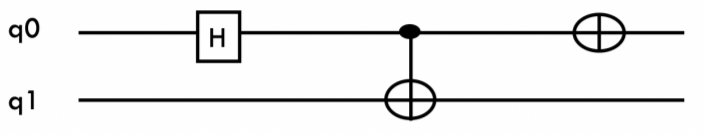
\includegraphics[scale=0.8]{figures/entanglement_statement.png}
\end{figure}

Comenzaremos estudiando un circuito ligeramente más sencillo que también produce entrelazamiento cuántico:

\begin{figure}[H]
	\centering
	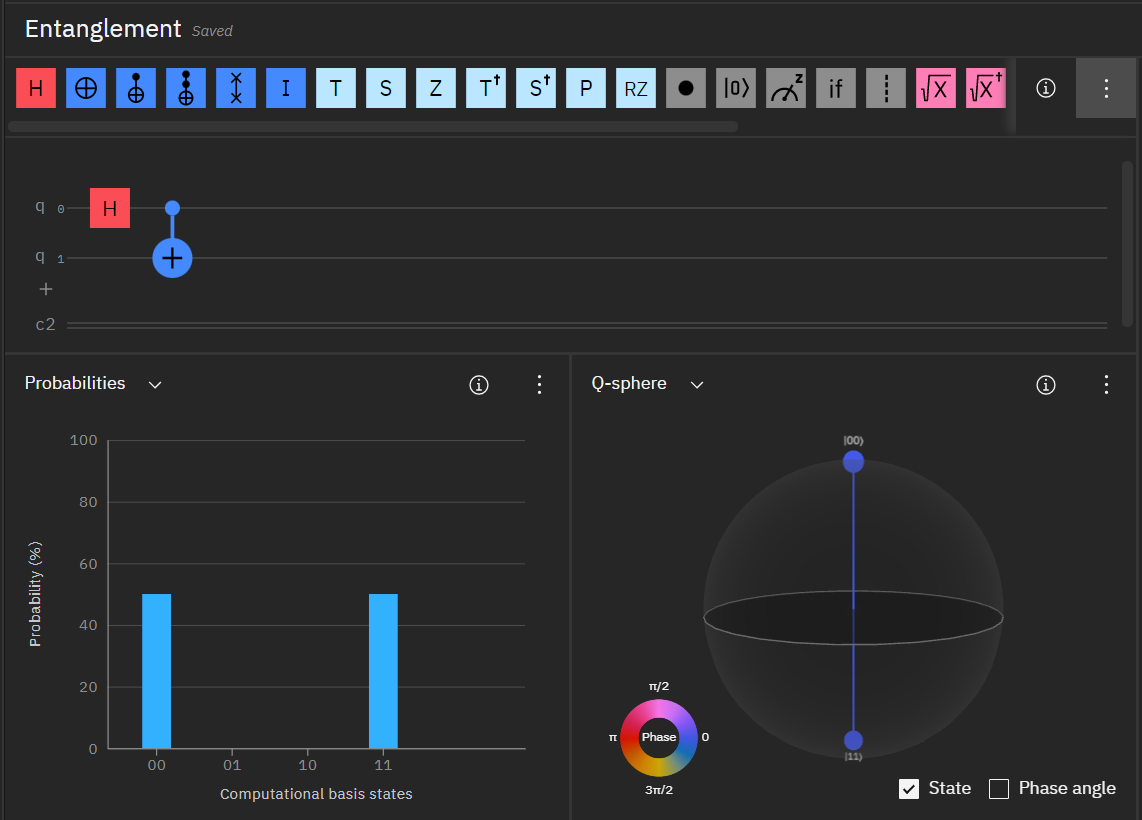
\includegraphics[scale=0.8]{figures/entanglement.png}
\end{figure}

Conociendo ya la puerta de Hadamard, sabemos que el resultado tras la aplicación de dicha puerta al estado $|0\ra$ será $|+\ra$. Utilizando a continuación de la puerta CNOT, como el estado de control tiene la misma probabilidad de ser $|0\ra$ que $|1\ra$, el segundo qubit tendrá la misma probabilidad de tener dichos valores. Analíticamente:

\[
	|+\ra|0\ra CNOT = \frac{|000\ra + |001\ra + |010\ra + |011\ra + |100\ra + |101\ra + |110\ra + |111\ra}{\sqrt 8} |0\ra
\]

\Phi



\subsection{Sumador de 2 qbits}



\section{Ejercicios opcionales de la práctica 2}

\end{document}
